%{{{Header
\documentclass[a4paper,11pt]{article}
\usepackage{anysize}
\marginsize{2cm}{2cm}{1cm}{1cm}
%\textwidth 6.0in \textheight = 664pt
\usepackage{xltxtra}
\usepackage{mathtools}
\usepackage{amsmath}
\usepackage{graphicx}
\usepackage{color}
\usepackage{xgreek}
\usepackage{framed}
\usepackage{float}
\usepackage{tkz-graph}
\usepackage{subfig}
\usepackage{fancyvrb}
\usepackage{minted}
\usepackage{listings}
\usepackage{hyperref}
\usepackage[noend]{algpseudocode}
\usepackage{algorithm}
\usepackage{enumitem}
\usepackage{relsize}
\setmainfont[Mapping=TeX-text]{DejaVu Serif}
\newcommand{\tab}{\hspace*{3em}}

%\setmainfont{Arial}
%\setsansfont{FreeSans}
%\setmonofont{FreeMono}
\begin{document}
%\def\thesubsection {\alph{subsection}}
\renewcommand{\labelenumi}{\roman{enumi})}
\renewcommand{\labelenumii}{ (\arabic{enumii}) }

\begin{titlepage}
\begin{center}
\begin{figure}[t]
     \includegraphics[scale=0.7]{title/ntua_logo}
\end{figure}
\begin{LARGE}\textbf{ΕΘΝΙΚΟ ΜΕΤΣΟΒΙΟ ΠΟΛΥΤΕΧΝΕΙΟ\\}\end{LARGE}
\vspace{5cm}
\begin{Large}
ΣΧΟΛΗ ΗΜ\&ΜΥ\\
Αλγόριθμοι και Πολυπλοκότητα\\
1\textsuperscript{η} Σειρά Γραπτών Ασκήσεων\\
Ακ. έτος 2010-2011\\
\end{Large}
\vspace{18cm}
\begin{tabular}{l r}

\begin{flushright}
\Large{Γερακάρης Βασίλης}\\
\large{Α.Μ.: 03108092}\\
\end{flushright}
\end{tabular}\\
\vspace{1cm}

\vfill
\large\today\\
\end{center}
\end{titlepage}


%}}}

%{{{ 1) Προβολή ταινιών
\section{Προβολή ταινιών} \setcounter{section}{1}
Θεωρούμε ότι οι k ταινίες αποτελούν τους κόμβους και τα n ζεύγη $(k_i, k_j)$
συμβολίζουν τις ακμές ενός μη-κατευθυνόμενου γραφήματος G. Τότε, το ερώτημα
του προβλήματος (να χωριστούν οι ταινίες σε 2 ημέρες, και να εμφανίζεται
ακριβώς 1 φορά έκαστη) ανάγεται σε έλεγχο διμερότητας του γραφήματος.

Επιλέγουμε (χωρίς βλάβη της γενικότητας) ένα τυχαίο κόμβο s και τον τοποθετούμε
στη λίστα του Σαββάτου. Εφαρμόζοντας BFS με αρχικό κόμβο τον s (επίπεδο i=0),
τοποθετούμε τους κόμβους που βρίσκονται σε άρτια επίπεδα ($i \mod 2 = 0$)
στη λίστα του Σαββάτου και τους κόμβους των περιττών επιπέδων στη λίστα της
Κυριακής.

Αν το γράφημα είναι συνεκτικό προχωράμε στο τελικό βήμα, ειδάλλως πρέπει να
επαναλάβουμε το BFS με αρχή έναν από τους ανεξερεύνητους κόμβους, εώς ότου
καλυφθούν όλες οι συνεκτικές συνιστώσες του γραφήματος.

Τέλος, εξετάζουμε τις n ακμές του γραφήματος:
\begin{itemize}
    \item Αν δεν υπάρχει ακμή με τα 2 άκρα της στην ίδια λίστα, το γράφημα
    είναι διμερές και η διαμέριση δίνεται από τις δημιουργημένες λίστες
    \item Αν υπάρχει τέτοια ακμή, το γράφημα περιέχει κύκλο περιττού μήκους
    και δε γίνεται να πραγματοποιηθεί η επιθυμητή διαμέρηση χωρίς να προβληθεί
    τουλάχιστον μία ταινία 2 φορές.
\end{itemize}

Η υπολογιστική πολυπλοκότητα της μεθόδου μας είναι $\Theta(k + n + n) =
O(k + n)$, αφού τόσο είναι το κόστος του BFS και ενός ελέγχου πάνω στις
ακμές.

%}}}

%{{{ 2) Μέτρηση συντομότερων μονοπατιών
\section{Μέτρηση Συντομότερων Μονοπατιών}
Για την επίλυση του ερωτήματος θα εφαρμόσουμε μια μικρή μετατροπή στον
αλγόριθμο του BFS: Κάθε κόμβος θα περιέχει ένα πεδίο στο οποίο θα αποθηκεύεται
το πλήθος των διαφορετικών τρόπων με τον οποίο μπορεί κανείς να φτάσει σε
αυτόν. Το πλήθος αυτό προκύπτει αθροίζοντας τις τιμές πλήθους από τους κόμβους
που βρίσκονται στο από πάνω επίπεδο και έχουν ακμή προς τον υπό εξέταση κόμβο.

\begin{algorithm}[H]
\caption{Shortest path counting}
\begin{algorithmic}[1]
\Procedure{cBFS}{$G(V,e)$}
\State $L[0] \gets s$
\State $C[s] \gets 1$
\State $i \gets 0$
\While {$L[i] \neq \emptyset$}
    \State $L[i+1] = \emptyset$
    \For{\textbf{each} $u \in L[i]$}
	\If {$u == target$}
	    \State \textbf{return} C[u]
	\EndIf
	\For{\textbf{each} $e \in G.incidentEdges(u)$}
	    \State $w \gets G.opposite(u,e)$
	    \If {$Discovered[w] == False$}
		\State $Discovered[w] \gets True$
		\State $L[i+1].append(w)$
	    \EndIf
	    \If {$w \notin L[i]$}
		\State $C[w] \gets C[w]+C[u]$
	    \EndIf
	\EndFor
    \EndFor
    \State $i \gets i+1$
\EndWhile
\EndProcedure
\end{algorithmic}
\end{algorithm}

Η πολυπλοκότητα του αλγορίθμου είναι $\Theta(m + n)$, αφού υλοποιεί ένα BFS.

Η ορθότητα προκύπτει λογικά, αφού το πλήθος των διαφορετικών μονοπατιών προς
ένα κόμβο ισούται με το άθροισμα των διαφορετικών μονοπατιών των κόμβων που
οδηγούν σε αυτό. Στην αλγοριθμική υλοποίηση του BFS που παρουσιάζεται
παραπάνω, η συνθήκη if (γραμμή 15) μας εξασφαλίζει ότι καταμετρούνται μόνο οι
ακμές από το παραπάνω επίπεδο και όχι οριζόντιες ακμές.
%}}}

%{{{ 3) Ελάχιστο Συνδετικό Δέντρο Υπό Περιορισμούς
\section{Ελάχιστο Συνδετικό Δέντρο Υπό Περιορισμούς (DVP 5.24)}
\subsection{Παράδειγμα}

\begin{figure}[ht]
    \centering
    \subfloat[Αρχικό γράφημα]{
	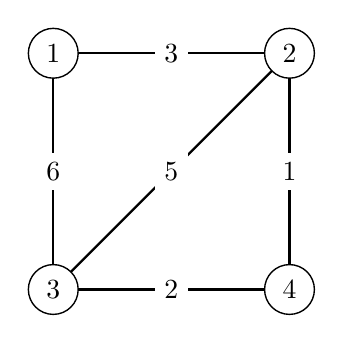
\begin{tikzpicture}
	    \Vertex[x=0,y=0,L=1]{1}
	    \Vertex[x=3,y=0,L=2]{2}
	    \Vertex[x=0,y=-3,L=3]{3}
	    \Vertex[x=3,y=-3,L=4]{4}

	    \Edge[label=3](1)(2)
	    \Edge[label=6](1)(3)
	    \Edge[label=5](2)(3)
	    \Edge[label=2](3)(4)
	    \Edge[label=1](2)(4)
	\end{tikzpicture}
    }
\hspace{1cm}
\subfloat[MST]{
    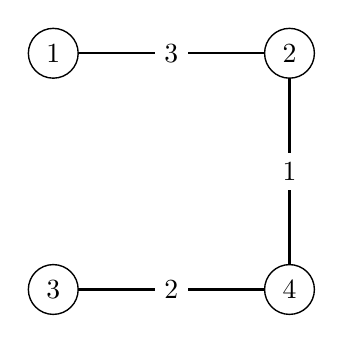
\begin{tikzpicture}
	\Vertex[x=0,y=0,L=1]{1}
	\Vertex[x=3,y=0,L=2]{2}
	\Vertex[x=0,y=-3,L=3]{3}
	\Vertex[x=3,y=-3,L=4]{4}

	\Edge[label=3](1)(2)
	\Edge[label=1](2)(4)
	\Edge[label=2](3)(4)
    \end{tikzpicture}
}
\hspace{1cm}
\subfloat[L = \{2\}]{
    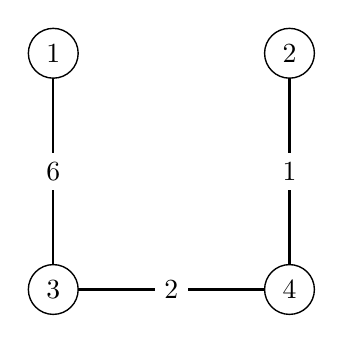
\begin{tikzpicture}
	\Vertex[x=0,y=0,L=1]{1}
	\Vertex[x=3,y=0,L=2]{2}
	\Vertex[x=0,y=-3,L=3]{3}
	\Vertex[x=3,y=-3,L=4]{4}

	\Edge[label=1](2)(4)
	\Edge[label=6](1)(3)
	\Edge[label=2](3)(4)
    \end{tikzpicture}
}
\end{figure}


\subsection{Αλγόριθμος}
Μπορούμε να επιλυσουμε το πρόβλημα με 2 τρόπους:
\begin{enumerate}
    \item Γνωρίζουμε ότι οι κορυφές που βρίσκονται στο L είναι φύλλα, επομένως
    είμαστε βέβαιοι ότι δε λειτουργούν συνδετικά ούτε δημιουργούν κύκλο.
    Μπορούμε οπότε να εφαρμόσουμε τον αλγόριθμο του Prim για να υπολογίσουμε
    το MST του γράφου G\textbackslash L σε χρόνο $\Theta (m + n \log n)$ και
    στη συνέχεια για κάθε κόμβο $u \in L$ επιλέγουμε την ελαχίστου κόστους
    ακμή που τον ενώνει με το MST που βρήκαμε (αποθηκεύοντας την προσωρινά,
    χωρίς να την προσθέσουμε ακόμα στο MST) σε χρόνο Ο(n).

    Όταν γίνει η επιλογή για όλους τους κόμβους του L, προσθέτουμε τις
    αποθηκευμένες ακμές στο MST και προκύπτει το επιθυμητό αποτέλεσμα σε
    χρόνο:\\
    $O(m + n \log n + n) = O(m + n \log n)$.\\
    \tab *(Η προσωρινή αποθήκευση γίνεται για την περίπτωση όπου ένας κόμβος
    $u_1 \in L$ προστεθεί στο MST και έπειτα η ελάχιστου κόστους ακμή ενός
    κόμβου $u_2 \in L$ είναι η $(u_1, u_2)$ και λανθασμένα επιλεγεί.)
    \item Δημιουργούμε το MST ακολουθώντας τον αλγόριθμο του Kruskal. Κάθε
    φορά, καθώς ψάχνουμε για κύκλο κρατάμε την τιμή της μέγιστου βάρους ακμής
    που βρίσκουμε. Αν βρεθεί κύκλος, κρατάμε την τιμή της διαφοράς (βάρος υπο
    εξέταση ακμής - βάρος μέγιστης ακμής) σε ένα πίνακα.

    Όταν τελειώσει η διαδικασία αυτή ο πίνακας θα περιέχει τα κόστη
    αναπλήρωσης για κάθε ακμή $e \notin MST$. Απο αυτά επιλέγουμε το μικρότερο
    και τοποθετούμε την ακμή στο MST, αφαιρώντας τη δεύτερη βαρύτερη στον
    κύκλο που θα σχηματιστεί. Η υλοποίηση αυτή έχει κόστος $\Theta (m \log m)$,
    αφού είναι παραλλαγή του αλγορίθμου του Kruskal.
    \end{enumerate}

%}}}

%{{{ 4) Μοναδικότητα Ελάχιστου Συνδετικού Δέντρου
\section{Μοναδικότητα Ελάχιστου Συνδετικού Δέντρου}
\subsection{}
Παρακάτω δίνεται παράδειγμα γράφου με ίδιο βάρος σε κάποιες ακμές που έχει
όμως μοναδικό MST. Επομένως το αντίστροφο δεν ισχύει.

\begin{figure}[ht]
    \centering
    \subfloat[Αρχικό γράφημα]{
	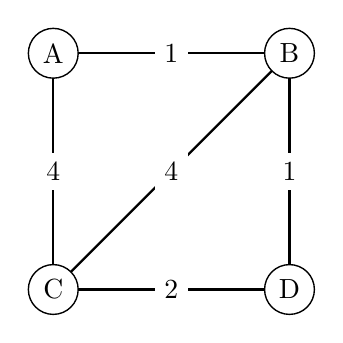
\begin{tikzpicture}
	    \Vertex[x=0,y=0,L=A]{A}
	    \Vertex[x=3,y=0,L=B]{B}
	    \Vertex[x=0,y=-3,L=C]{C}
	    \Vertex[x=3,y=-3,L=D]{D}

	    \Edge[label=1](A)(B)
	    \Edge[label=4](A)(C)
	    \Edge[label=4](B)(C)
	    \Edge[label=2](C)(D)
	    \Edge[label=1](B)(D)
	\end{tikzpicture}
    }
\hspace{1cm}
\subfloat[MST]{
    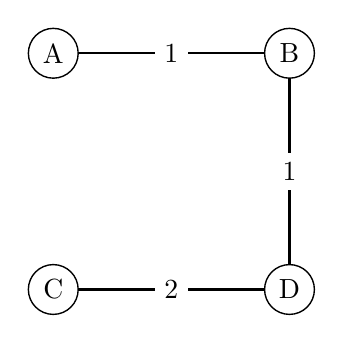
\begin{tikzpicture}
	\Vertex[x=0,y=0,L=A]{1}
	\Vertex[x=3,y=0,L=B]{2}
	\Vertex[x=0,y=-3,L=C]{3}
	\Vertex[x=3,y=-3,L=D]{4}

	\Edge[label=1](1)(2)
	\Edge[label=1](2)(4)
	\Edge[label=2](3)(4)
    \end{tikzpicture}
}
\end{figure}

\subsection{}
Θα το αποδείξουμε με εις άτοπον απαγωγή. Έστω ότι το MST T, δεν είναι
μοναδικό, δηλαδή υπάρχει ένα δέντρο T' με ίδιο βάρος ακμών. Αφού είναι
διαφορετικά, θα υπάρχει τουλάχιστον μία τομή του γραφήματος, όπου η ακμή
e του T και η e' του Τ' θα είναι διαφορετικού βάρους (χωρίς βλάβη της
γενικότητας, με $e < e'$). Προσθετοντας την e στο Τ' δημιουργείται κύκλος που
περιέχει τις e, e' . Το δέντρο $T' \cup \{e\} \backslash \{e'\}$ παραμένει
συνδετικό και έχει βάρος $|T'| - e' + e < |T|$. Επομένως μπορούμε να
κατασκευάσουμε ένα καλύτερο MST, πράγμα άτοπο, αφού υποθέσαμε ότι το Β ήταν
MST (άρα ελάχιστο εξ'ορισμού).

Το αντίστροφο δεν ισχύει, όπως φαίνεται και από το παράδειγμα του 1ου
ερωτήματος. Η τομή που χαρακτηρίζεται από τις ακμές (Α,Β),(Β,Γ),(Β,Δ) έχει
ακμές ίδιου βάρους αλλά το MST είναι μοναδικό.
\subsection{Συνθήκη}
Η ικανή και αναγκαία συνθήκη για να υπάρχει μοναδικό MST ενός γράφου G έχει 2
συνιστώσες:
\begin{itemize}
    \item Για κάθε διαμέριση των κόμβων του G σε 2 συνεκτικές συνιστώσες, η
    ελαχίστου βάρους ακμή με άκρα σε αμφότερα τα υποσύνολα είναι μοναδική.
    \item Η μεγίστου βάρους ακμή σε κάθε κύκλο του G είναι μοναδική.
\end{itemize}

Το $1^o$ μέρος της απόδειξης έγινε προηγουμένως, ότι δηλαδή καμία από τις ακμές
που χωρίζουν το γράφημα σε 2 συνεκτικές συνιστώσες, δε γίνεται να
αντικατασταθεί από κάποια άλλη.

Το αντίστροφο (δηλαδή το ότι αν υπάρχει μοναδικό MST, τότε δε γίνεται να
αντικατασταθεί καμία από τις ακμές του με άλλη) προκύπτει από τη λειτουργία
του αλγορίθμου του Prim: Στην περίπτωση που 2 συνεκτικές συνιστώσες του
γραφήματος συνδέονταν με 2 ακμές ίδιου βάρους, ο αλγόριθμος του Prim θα επέλεγε
τυχαία κάποια από τις 2, οπότε δε θα είχαμε μοναδικό MST.

\subsection{Αλγόριθμος}
Ένας αλγόριθμος με πολυπλοκότητα $O(|V|^2)$ είναι ο εξής:

Εφαρμόζουμε BFS στο MST και αποθηκεύουμε το βάρος της βαρύτερης
τιμής για κάθε μονοπάτι $(u_1,u_2)$ σε ένα πίνακα μεγέθους $V^2$. \\
Για κάθε τομή του G που τον χωρίζει σε 2 συνεκτικές συνιστώσες, συγκρίνουμε
τις τιμές των ακμών που τη διασχίζουν με την τιμή που βρίσκεται στον πίνακα.

Αν προκύψει ισότητα, τότε το MST δεν είναι μοναδικό, ειδάλλως, αν ολοκληρωθεί
η διαδικασία τότε το MST του γραφήματος είναι μοναδικό.
%}}}

%{{{ 5) Υπολογισμός ελάχιστου συνδετικού δέντρου με διαγραφή ακμών
\section{Υπολογισμός Ελάχιστου Συνδετικού Δέντρου με Διαγραφή Ακμών}
\begin{enumerate}
\item Στο παρακάτω παράδειγμα φαίνεται πως η ακμή e μέγιστου βάρους (5) που
βρίσκεται στον κύκλο B->C->D->B δεν περιέχεται στο MST.
\begin{figure}[ht]
    \centering
    \subfloat[Αρχικό γράφημα]{
	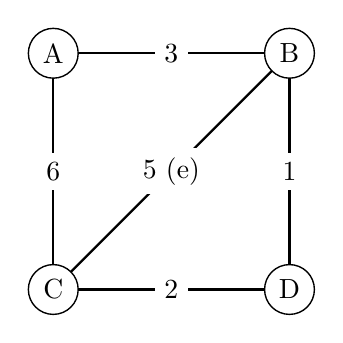
\begin{tikzpicture}
	    \Vertex[x=0,y=0,L=A]{A}
	    \Vertex[x=3,y=0,L=B]{B}
	    \Vertex[x=0,y=-3,L=C]{C}
	    \Vertex[x=3,y=-3,L=D]{D}

	    \Edge[label=3](A)(B)
	    \Edge[label=6](A)(C)
	    \Edge[label=5 (e)](B)(C)
	    \Edge[label=2](C)(D)
	    \Edge[label=1](B)(D)
	\end{tikzpicture}
    }
\hspace{1cm}
\subfloat[MST]{
    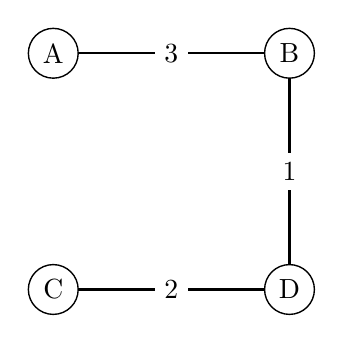
\begin{tikzpicture}
	\Vertex[x=0,y=0,L=A]{1}
	\Vertex[x=3,y=0,L=B]{2}
	\Vertex[x=0,y=-3,L=C]{3}
	\Vertex[x=3,y=-3,L=D]{4}

	\Edge[label=3](1)(2)
	\Edge[label=1](2)(4)
	\Edge[label=2](3)(4)
    \end{tikzpicture}
}
\end{figure}

\item
    \begin{enumerate}
	\item Αρχικά, ο παραπάνω αλγόριθμος είμαστε βέβαιοι ότι θα υπολογίσει
	ένα spanning tree, γιατί αφαιρεί μόνο τις ακμές που
	δημιουργούν κύκλους στο γράφημα. Το τελικό αποτέλεσμα θα είναι ένα
	δέντρο (αφού δεν περιέχει κύκλους) το οποίο θα είναι και συνδετικό,
	αφού η διαδικασία διαγραφής ακμών δεν επιτρέπει διαγραφή ακμών που θα
	καταστήσουν το γράφημα μη-συνεκτικό.
	\item Επιπλέον το συνδετικό δέντρο T που προκύπτει θα είναι και
	ελάχιστο.\\ Έστω ότι δεν ήταν ελάχιστο, αυτό σημαίνει ότι θα μπορούσε
	κάποιος να προσθέσει κάποια ακμή $e_1$ που θα δημιουργούσε κύκλο και
	αφαιρώντας μία άλλη, $e_2$ μεγαλύτερου κόστους θα κατέληγε σε MST.

	Αυτό είναι άτοπο, αφού ο αλγόριθμος που περιγράφηκε θα επέλεγε για
	διαγραφή την $e_2$, όταν έφτανε στον κύκλο που περιείχε τις $e_1$ και
	$e_2$.
    \end{enumerate}
\item
Μία αποδοτική υλοποίηση θα ήταν ο αλγόριθμος του Kruskal με φθίνουσα
ταξινόμηση στο βάρος των ακμών. Ακολουθώντας τη λογική του αλγορίθμου που
περιγράφηκε προκύπτει η παρακάτω μορφή του αλγορίθμου:

\begin{algorithm}[H]
\caption{Άσκηση 5}
\begin{algorithmic}[1]
\Procedure{Deletion\_MSP}{G(V,e,w)}
\State Sort edges by decending weight
\State $T \gets G$
\For {\textbf{each} $e_i \in G$}
    \If {$\{e_i\}$ belongs in cycle}
	\State $T \gets T - \{e_i\}$
    \EndIf
\EndFor
\EndProcedure
\end{algorithmic}
\end{algorithm}

Η υλοποίηση του αλγορίθμου του Kruskal με χρήση BFS για τον έλεγχο
κύκλων απαιτεί χρόνο $O(m(m+n)) = O(m^2)$ .

\end{enumerate}

%}}}

\end{document}
